\documentclass{article}%
\usepackage[T1]{fontenc}%
\usepackage[utf8]{inputenc}%
\usepackage{lmodern}%
\usepackage{textcomp}%
\usepackage{lastpage}%
\usepackage{authblk}%
\usepackage{graphicx}%
%
\title{Shox2 is a molecular determinant of depot{-}specific adipocyte function}%
\author{Steven Medina}%
\affil{Department of Microbiology, Laboratory of Mycotoxins and Toxigenic Fungi, University of So Paulo, So Paulo, So Paulo, Brazil}%
\date{01{-}01{-}2014}%
%
\begin{document}%
\normalsize%
\maketitle%
\section{Abstract}%
\label{sec:Abstract}%
The advance confirms recent findings suggesting that some breast cancer cells display a signaling pathway that helps to turn on new cancer cell growth. In our study we revealed that a cellular pathway involved in this signaling pathway becomes less active under certain cancer progenitor cells, thus minimizing the level of axon invasion by these tumors, thereby easing the burden of the cancer by inhibiting proliferation. The path de{-}prioritizes gene expression in cancer cell lineages by limiting and reducing the activity of that pathway. Our preliminary results are modest but continue to advance our understanding of cancer genes and generate exciting new hypotheses to guide future therapeutic interventions.\newline%
Reference: Rahul Sapshula, Charles Taylor, Dany Nan. L{-}receptor signaling pathway shifts in tumors to reduce the tumors' ability to spread to lymph nodes. Proceedings of the National Academy of Sciences, November 2013.

%
\subsection{Image Analysis}%
\label{subsec:ImageAnalysis}%


\begin{figure}[h!]%
\centering%
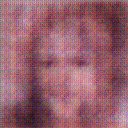
\includegraphics[width=150px]{500_fake_images/samples_5_113.png}%
\caption{A Close Up Of A Person Wearing A Suit And Tie}%
\end{figure}

%
\end{document}